\documentclass[openany]{memoir}
\usepackage[utf8]{inputenc}
\usepackage[czech]{babel}
\usepackage[T1]{fontenc}
\usepackage{amsmath}
\usepackage{amsfonts}
\usepackage{amssymb}
\usepackage[top=-2cm, bottom=2cm, left=2cm, right=2cm]{geometry}
\usepackage{fancyhdr}
\usepackage{graphicx}
\usepackage{lmodern}
\usepackage{xwatermark}
\usepackage{xcolor}
\usepackage{leadsheets}%http://mirrors.nic.cz/tex-archive/macros/latex/contrib/leadsheets/leadsheets_en.pdf   --> dokumentace	
\definesongtitletemplate{empty}{} 
\setchords{
format = \bfseries,
minor = {mi},%
input-notation = {german},%
output-notation = {german}%
}

\chapterstyle{bianchi}  %ALT BIANCHI, veelo

\newlength{\drop}
\newwatermark[allpages,color=red!50,angle=0,scale=2, xpos=0,ypos=0]{
\includegraphics[width=5cm]{obr/dvojka.jpg}} %--> dvojk av pozadí


\setleadsheets{
  title-template = empty ,
  chords/sharp = \# ,
  chords/flat = b
}


%--> Pozn. Noty se vždycky lepí na slovo, které je těsně u nich. Nemůžou tedy být mezi dvěma slovy. Taky mezi slovem a \\ musí být mezera


\begin{document}

\thispagestyle{empty}
\mainmatter
\thispagestyle{empty}
\newpage 
{ \vspace*{4cm}

   \drop=0.1\textheight
    \centering
    
    \vspace*{\baselineskip}
    \scshape
2017
    \rule{\textwidth}{1.6pt}\vspace*{-\baselineskip}\vspace*{2pt}
    \rule{\textwidth}{0.4pt}\\[\baselineskip]
    {\LARGE Dvojkařský zpěvník}\\[0.2\baselineskip]
    \rule{\textwidth}{0.4pt}\vspace*{-\baselineskip}\vspace{3.2pt}
    \rule{\textwidth}{1.6pt}\\[\baselineskip]
    \scshape
\vspace{3.2cm}
 }  

\begin{figure}[h]
\centering
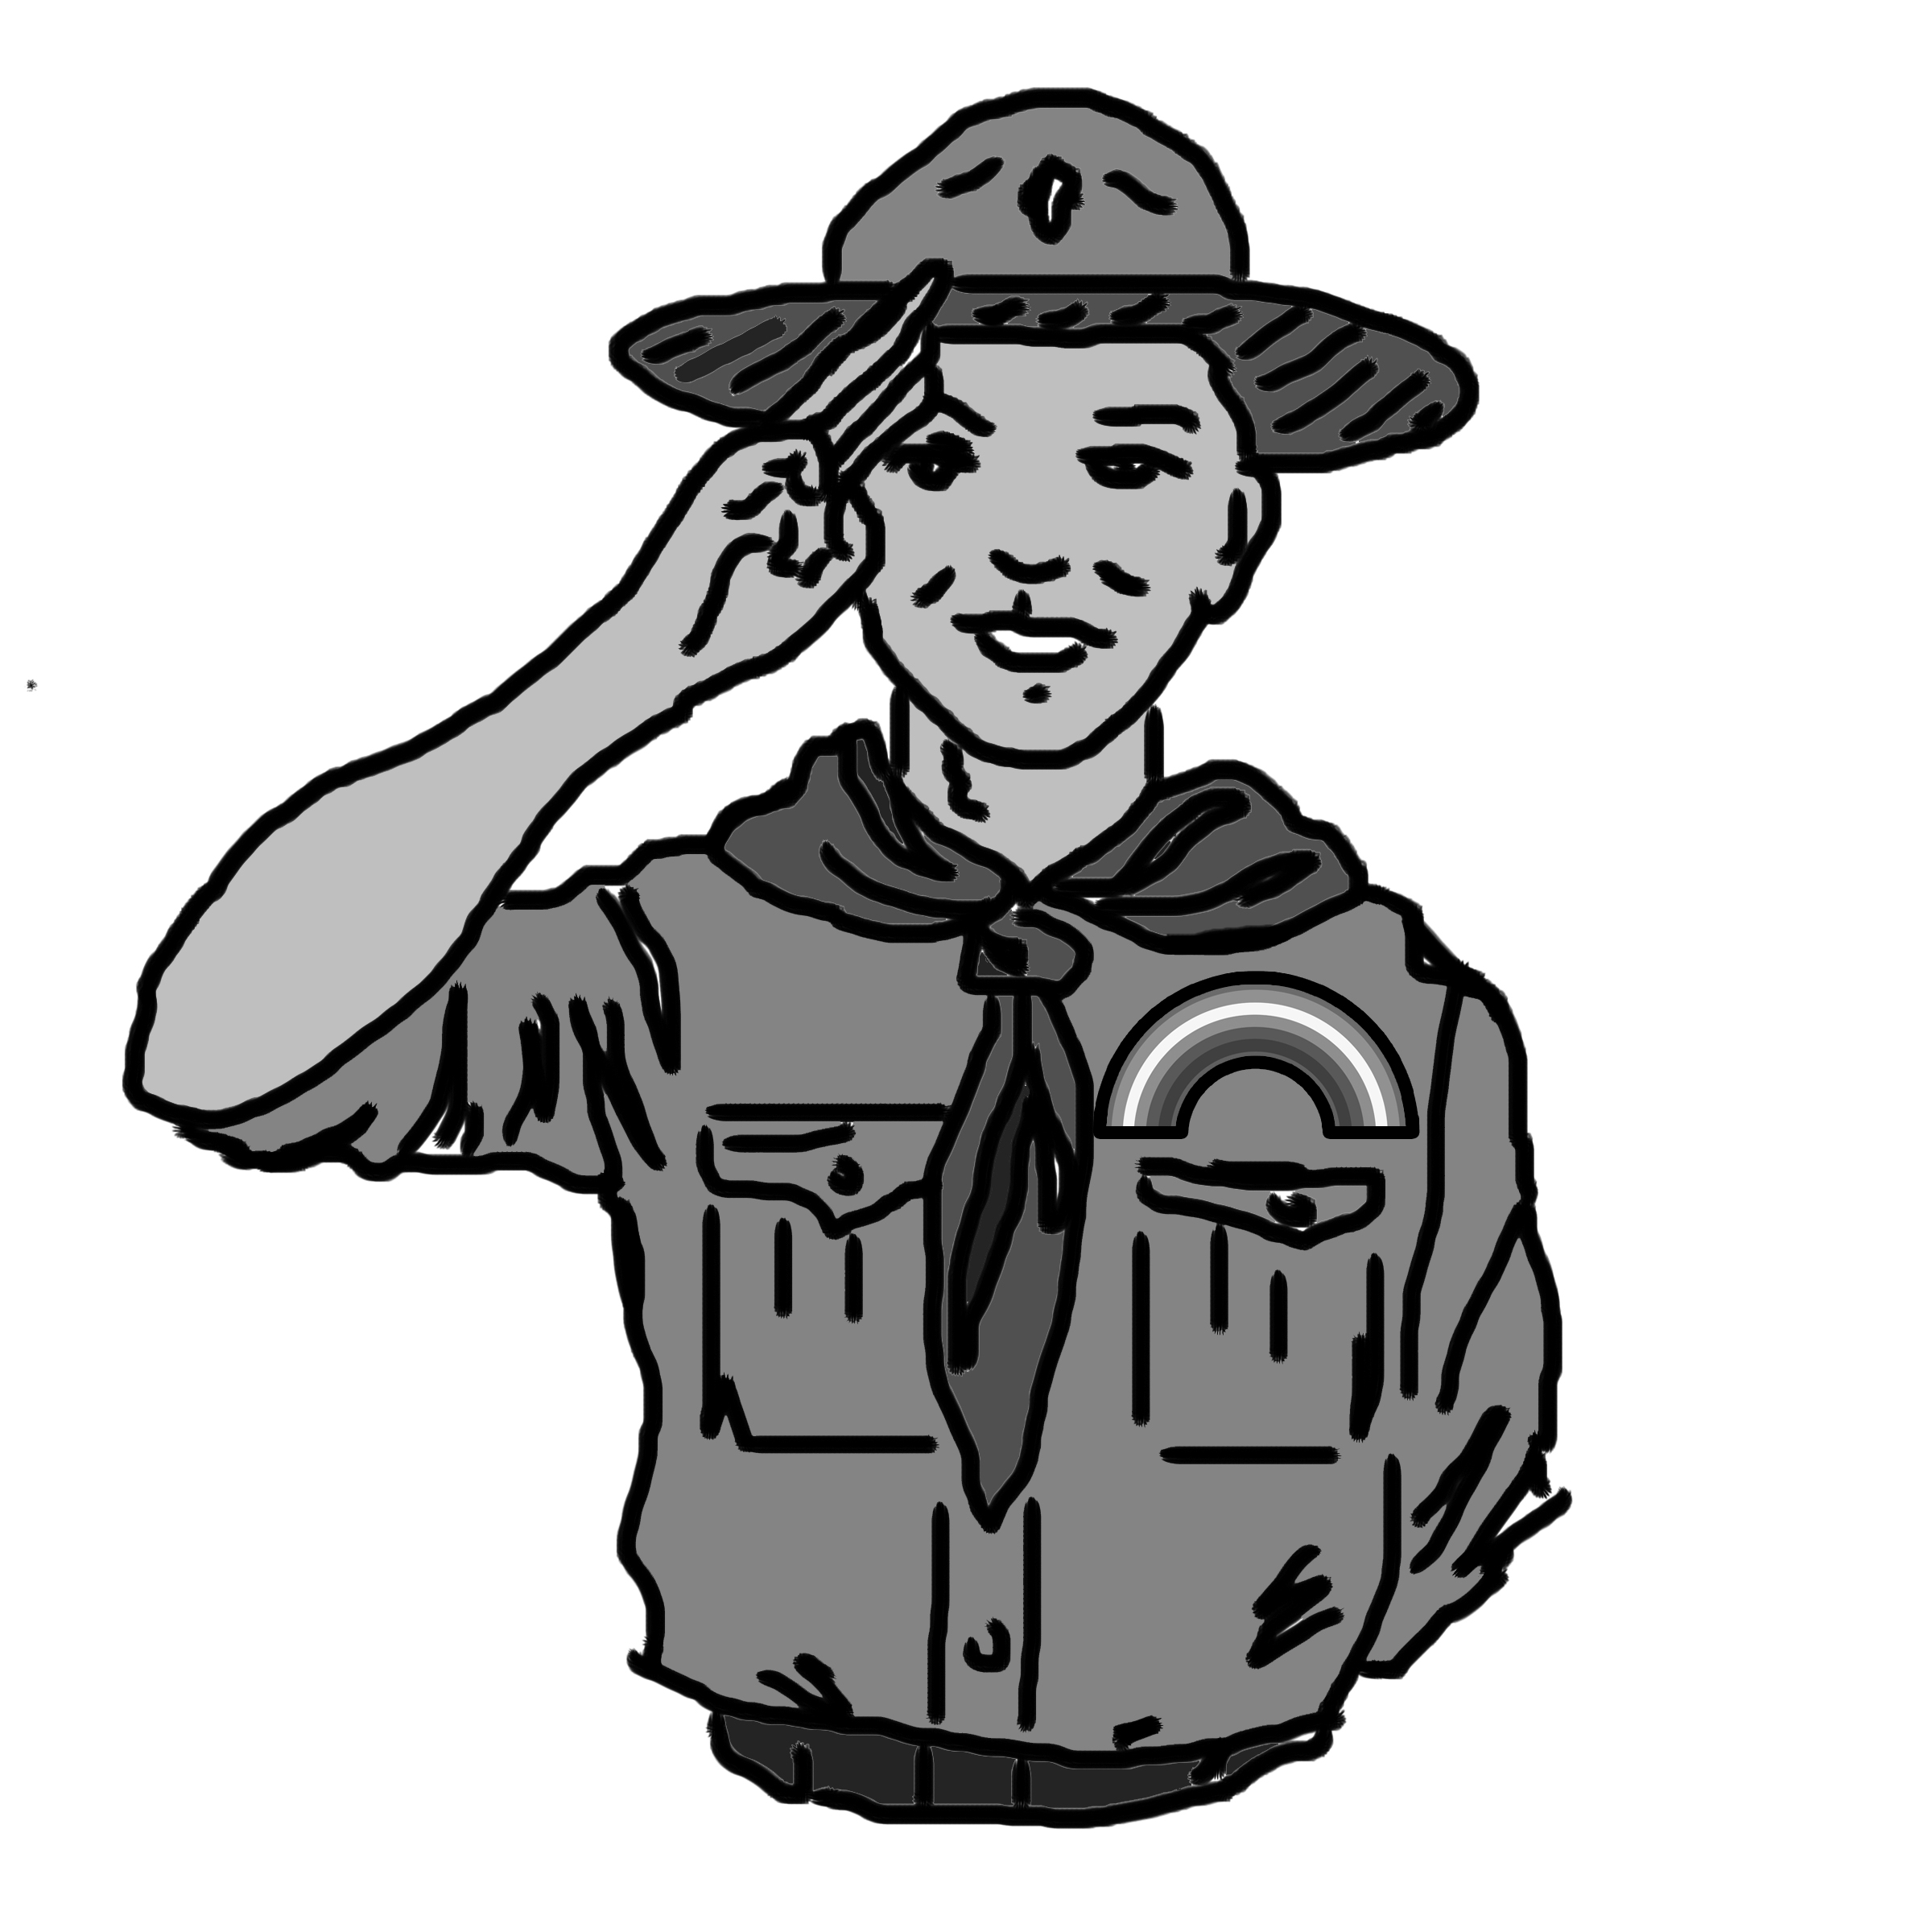
\includegraphics[scale=0.6]{obr/boyscout.jpg}
\end{figure}
\newpage
\tableofcontents

\chapter{Do Ameriky}

\noindent\hspace{0.15\linewidth}\begin{minipage}{0.7\linewidth}

\begin{song}{title=Do Ameriky}

\begin{verse}[numbered]
^{D}Do Ameriky jezděj Parníky,\\
když tam přijdeš, zdá se ti to ^{A7}všecko veliký,\\
^{\phantom{S}}je to fakticky hodně praktický  \\
přijít tam a umět anglic^{D}ky. \\
\end{verse}
\begin{verse*}
\hspace*{-0.45cm}\textbf{R:} 
^{D}Dobrou noc - good night, ^{A7}výborně - all right,\\
Konrád White, už je off^{D}side (housemister - Dally sister!) \\
^{D}Dneska je today, ^{A7}dobrý den - good day,\\
já jsem byl taky chu^{D}dej. \\ 
^{G}His Master's Voice, Yankee Doo^{G}dle,\\ \\
^{En7}máš apetit? (mám) ^{A7}vem si štrůdl! (do pusy)\\
^{D}Sto kilo je cent, ^{A7}patent je patent,\\
husa v troubě happy^{D}end.
\end{verse*}
\begin{verse}[numbered]
Co Buffalo Bill vrazil do kobyl,\\
za to by si bejval byl koupil automobil,\\
cowboy na koni už se nehoní,\\
přestože mu Fordka nevoní.\\
\end{verse}
\begin{verse*}
\hspace*{-0.45cm}\textbf{R:} 
\end{verse*}
\begin{verse}[numbered]
Mám na západě chajdu v Nevadě,\\
zlatou žílu v Arizoně, doly v Kanadě,\\
babička na mě šetří v Panamě\\
ačkoli tu žiju náramě!\\
\end{verse}
\end{song}
\end{minipage}


\chapter{Hey Ho, Nobody's Home}
\noindent\hspace{0.15\linewidth}\begin{minipage}{\linewidth}
\begin{song}{title=Pangajó}

\begin{verse}[numbered]
^{Ami}Hey ^{Emi}ho, ^{Ami}nobodys ^{Emi}home, \\
^{Ami}meat nor ^{Emi}drink nor ^{Ami}money have I^{Emi}none. Yet \\
^{Ami}Every ^{Emi}time I ^{Ami}will be ^{Emi}happy. \\
/: ^{Ami}Zum gali ^{Emi}gali gali, ^{Ami}zum gali^{Emi}gali. :/\\
\end{verse}
\end{song}
\end{minipage}

\chapter{Je Jaká Je \\ \huge{Karel Gott}}
\noindent\hspace{0.15\linewidth}\begin{minipage}{0.7\linewidth}
\begin{song}{title=Pangajó}

\begin{verse}[numbered]
^{D} Je ja ^{F#mi} ká je, ^{G}tak mi náh ^{A} le padla ^{D}do k ^{F#mi} lína, \\
^{G} ani ^{A} černá ^{D} ani blo ^{F#mi} ndýna, ^{G} někdy ^{A} tak a jin ^{D} dy taková, \\
^{Hmi} ^{G} vždyc ^{A} ky hádam jak ^{D} se ^{Hmi} zacho ^{G} vá, ^{A} zrejme nik ^{D} dy ^{Hmi} jak ^{G} ch ^{A} ci já.
\end{verse}
\begin{verse}[numbered]
Je jaká je, trochu dítě, trochu mondéna, \\
nemám právě paměť na jména, tak jí říkám lásko má. \\
Nejsi skvost a nejsi zlá, jsi jen jiná než chci já. \\
\end{verse}
\begin{verse}[numbered]
Je jaká je, že se změní čekat nedá se, \\
snad jí záleží jen na kráse, tak, že člověk málem nedutá, \\
jak je štíhlá, jak je klenutá, jenže jinak, než chci já. \\
\end{verse}
\begin{verse}[numbered]
Je jaká je, až jí zitra spatříš u pláže, \\
vzkaž jí, ať se na mě neváže, ať si pro mě vrásky neděla, \\
ať je jaká je a veselá, i když jiná než chci já. \\
\end{verse}
\end{song}
\end{minipage}

\chapter{Kamarádi \\ \huge{Poslední výstřel}}
\noindent\hspace{0.15\linewidth}\begin{minipage}{0.7\linewidth}
\begin{song}{title=Pangajó}

\begin{verse}[numbered]
 ^{Emi} Bývaly chvíle kdy jsem ^{G} chtěl sundat \\
brýle a ^{Ami} říct ti: \uv{Pojď ^{C} ven}. \\ 
Pak jsem to ale nějak překousl \\
ač jsi mě rozhněval hodně \\
\end{verse}
\begin{verse}[numbered]
Bývaly chvíle kdy mi nebylo milé, \\
že patřím k takovým lidem \\
Ne, ne, kámoše si nevybereš \\
Kámoš je ten, kdo na tebe zbyde \\
\end{verse}
\begin{verse*}
\hspace*{-0.45cm}\textbf{R:}  (akordy stejné jak ve sloce)\\
Pořád jsme kamarádi, pořád jsme kamarádi \\
Pořád jsme kamarádi, pořád jsme kamarádi \\
Co jsme si, to jsme si, co jsme si, to jsme si \\
pořád jsme kamarádi \\
Co jsme si, to jsme si, co jsme si, to jsme si, \\
pořád jsme kamarádi
\end{verse*}
\begin{verse}[numbered]
Bývaly chvíle, kdy sis chtěl sundat \\
brýle a říct mi: \uv{Pojď ven} \\
Pak jsi to ale nějak překousl \\
ač jsem tě rozhněval notně
\end{verse}
\begin{verse}[numbered]
Bývaly chvíle kdy ti nebylo milé \\
že patříš k takovým lidem \\
Kámoše si prostě nevybereš \\
kámoš je ten kdo na tebe zbyde 
\end{verse}
\begin{verse*}
\hspace*{-0.45cm}\textbf{R:} 
\end{verse*}
\end{song}
\end{minipage}

\chapter{Knockin' On The Heaven's Door \\ \huge{Bob Dylan}}
\noindent\hspace{0.15\linewidth}\begin{minipage}{0.7\linewidth}
\begin{song}{title=Pangajó}

\begin{verse}[numbered]
 ^{G} Mama, ^{D} take this badge off of me ^{Ami} \\
 ^{G} I can't ^{D} use it anymore ^{C}. \\
It's gettin' dark, too dark for me to see \\
I feel like I'm knockin' on heaven's door.
\end{verse}
\begin{verse*}
\hspace*{-0.45cm}\textbf{R:} ^{G} Knock, knock \\
 ^{D} knockin' on heaven's  ^{Ami} door \\
 ^{G} Knock, knock, \\
 ^{D} knockin' on heaven's ^{C} door \\
Knock, knock, knockin' on heaven's door \\
Knock, knock, knockin' on heaven's door \\
\end{verse*}
\begin{verse}[numbered]
Mama, put my guns in the ground \\
I can't shoot them anymore. \\
That long black cloud is comin' down \\
I feel like I'm knockin' on heaven's door. 
\end{verse}
\begin{verse*}
\hspace*{-0.45cm}\textbf{R:}Knock, knock, knockin' on heaven's door \\
Knock, knock, knockin' on heaven's door \\
Knock, knock, knockin' on heaven's door \\
Knock, knock, knockin' on heaven's door
\end{verse*}
\end{song}
\end{minipage}

\chapter{Kutil \\ \huge{Chinaski}} 
\noindent\hspace{0.15\linewidth}\begin{minipage}{0.7\linewidth}
\begin{song}{title=Pangajó}

\begin{verse}[numbered]
Jsem ^{E} kutil \\
mám malou ^{F#mi} dílnu víc ^{A} mě nezají ^{E} má \\
mé ^{E} hobby je moje práce \\
šťastnej ^{F#mi} člověk kaž ^{A} dej kdo to tak ^{E} má \\
mám ^{E} ženu \\
 je mladá ^{F#mi} krásná chyt ^{A} rá přívěti ^{E} vá \\
má jednu malinkatou ^{E} chybu \\
že si ^{F#mi} se mnou vů ^{A} bec nepoví ^{E} dá\\
\end{verse}
\begin{verse*}
\hspace*{-0.45cm}\textbf{R:}  Atak ^{F#mi} hledám holku sdílnou \\
co by chtěla kluka s dílnou \\
^{A} abych nebyl ^{H}sám ^{H7}
\textbf{E  F#mi  A  E  C#mi  A  G  D  E } 
\end{verse*}
\begin{verse}[numbered]
Jsem kutil \\
mám malou dílnu víc mě nezajímá \\
má práce je moje hobby \\
šťastnej člověk každej kdo to tak má \\
mám ženu \\
je mladá krásná chytrá přívětivá \\
má jednu malinkatou chybu \\
že si se mnou vůbec nepovídá
\end{verse}
\begin{verse*}
\hspace*{-0.45cm}\textbf{R:} 
\end{verse*}
\end{song}
\end{minipage}

\chapter{Milionář \\ \huge{Jaromír Nohavica}}

\noindent \begin{minipage}{0.5\linewidth}
\begin{song}{title=Pangajó}

\begin{verse}[numbered]
^{D}U nás v domě ^{A} říkají mi Franta Šiš ^{D} ka\\
bo už od pohledu ^{G}  chytry jsem jak liš ^{D} ka \\
a dyž ^{A}  kery něco neví \\
nebo ^{D} dyž je na co levy  \\
tak de za ^{Emi} mnu a ja ^{A} všecko najdu v kni ^{D} žkach 
\end{verse}
\begin{verse}[numbered]
Raz mi říkal jeden znamy dole v baře \\
že s tu hlavu moh bych do Milionaře \\
čemu ne říkám si brachu \\
šak má Železný dost prachu \\
no a Čechovi se podíváš do tvaře 
\end{verse}
\begin{verse}[numbered]
Dostal jsem se mezi partu uchazeču \\
nikdo nemá šajnu jak tam nervy teču \\
všecko viděl jsem do hnědě \\
tak jsem zmáčknul AbeCeDe \\
no a už mě kruci ke stolečku vleču 
\end{verse}
\begin{verse}[numbered]
Čech to začal takym malym interviju \\
co pry robim esi kuřim a co piju \\
tak jsem řeknul co jsem řeknul \\
on se evidentně leknul \\
a už začly blikat světla ve studiu
\end{verse}
\begin{verse}to se přiznam nebylo mi vesele
První otázka pry co je ukulele \\
tož tak jsem radši hlavu sklonil \\
abych to všecko nezkonil \\
říkám chtěl bych se obratit na přitele 
\end{verse}
\begin{verse}[numbered]
Lojza byl po hlasu silně nevyspaly \\
asi zase celu šichtu prochlastali \\
bylo slyšet jak tam dycha \\
ale třicet vteřin ticha \\
to je tak dyž se vam kamarad navali.
\end{verse}
\begin{verse}[numbered]
Moju staru zatím doma braly mory \\
lidi ohryzavali televizory \\
\end{verse}
\end{song}
\end{minipage}
\begin{minipage}{0.5\textwidth}
\begin{itemize}
\item[] tady nešlo nad čim plesat \\
tož padesat na padesat \\
ať vím esi su to ty bulharské hory\\
\item[8.] A už jasně na tym komputuře sviti \\
buďto je to za A vzacne lučni kviti \\
nebo za Be nastroj strunny \\
tu de kurňa o koruny \\
a ja stejně jak na začatku jsem v řiti \\
\item[9.] Čech tam zatím maval tymi svymi čisly \\
tak si řikam Franta napij sa a mysli \\
jake tudy sakypaky \\
obratiš se na divaky\\
šak tu zatím za ty prachy enem kysli \\
\item[10.] Sam jsem byl zvědavy co publikum zvoli \\
bo aj v obecenstvu možu sedět voli \\
devadesat procent za Be \\
ale to mi přišlo slabe \\
bo co není stopro to mě dycky smali \\
\item[11.] Ještě že jsem chlap co zboja neutika \\
říkam pane Čechu pujdem do rizika \\
měl jsem v gaťach nadělano \\
ale Čech zakřičel ano \\
mate pravdu je to nastroj hudebnika \\
\item[12.] Lidi tleskali bo uspech to byl plny \\
radosti zrobili dvě mexicke vlny \\
a ja co mam srdce skromne \\
jako všeci z Dolni Lomne \\
jsem byl spokojeny bo sem ukol splnil \\
\item[13.] Pane Čechu nerad přetahnul bych strunu \\
končim hru a beru tisicikorunu \\
Čech se jenom chytnul stolu \\
obočí mu spadlo dolu \\
no a už se modry ku podlaze sunul \\
\item[14.] První třidu do Ostravy Intercity \\
v jidelňaku celu cestu valim kyty \\
a ta stovka co mi zbude \\
to je přispěvek na chude \\
bo Ostrava je region razovity.
\end{itemize}
\end{minipage}

\chapter{Ostravo, Ostravo \\ \huge{Jaromír Nohavica}}
\noindent\hspace{0.15\linewidth}\begin{minipage}{0.7\linewidth}
\begin{song}{title=Pangajó}

\begin{verse*}
\hspace*{-0.45cm}\textbf{R:} ^{Dmi} Ostravo, Ostra ^{A7} vo, \\
město mezi městy, ^{Dmi} hořké ^{A7} moje štěstí. \\
^{Dmi} Ostravo, Ostra ^{A7} vo, \\
černá hvězdo nad hla ^{Dmi} vou.
\end{verse*}
\begin{verse}[numbered]
^{C} Pán Bůh rozdal jiným ^{F} městům všecku krásu, \\
^{Gmi} parníky na řekách a ^{A7} dámy všité do atlasu. \\
^{Dmi} Ostravo - srdce ru ^{A7} dé,\\
zpečetěný osu ^{D} mide. ^{A7}  ^{Dmi}
\end{verse}
\begin{verse*}
\hspace*{-0.45cm}\textbf{R:}
\end{verse*}
\begin{verse}[numbered]
Ať mě moje nohy nesly, kam mě nesly, \\
ptáci na obloze jenom jednu cestu kreslí.\\
Ostravo - srdce rudé,\\
zpečetěný osude.
\end{verse}
\end{song}
\end{minipage}

\chapter{Osmá Barva Duhy}


\chapter{Pangajó}
\noindent\hspace{0.15\linewidth}\begin{minipage}{0.7\linewidth}
\begin{song}{title=Pangajó}

\begin{verse}[numbered]
^{Ami}Pangajo, Pangajo \\
^{Dmi}ka mudi ^{Ami}ka \\
rodi ^{G}he rodi hu \\
arong ^{Ami}baina ^{G}pondi ^{Ami}he  \\
te hu ^{G}a kema ^{Ami}o  \\
Te hu ^{G}a kema ^{Ami}o aó aó aó \\
\end{verse}
\end{song}
\end{minipage}


\chapter{Převrat V Banánové Republice\\ \huge{Znouzecnost}}
\noindent\hspace{0.15\linewidth}\begin{minipage}{0.7\linewidth}
\begin{song}{title=Pangajó}

\begin{verse}[numbered]
^{F}Generál ^{C}Sancho ^{B}Grácia ^{C}zmocnil ^{F}se vlády ^{C} ^{B} ^{C} \\
v Banánový republice někde uprostřed pralesa. \\
Hlásili to po ránu ve zprávách a psali v novinách, \\
Banánová republika, kde není nic jinýho než banány ^{F}a ^{C}armáda ^{B} ^{C}
\end{verse}
\begin{verse*}
\hspace*{-0.45cm}\textbf{R:}  ^{Dmi}A já vám ^{B} řikam, že ^{C}z tohodle nekouká ^{F} zas nic ^{C} dobrý ^{Dmi} ho \\
^{Dmi}A já vám ^{B} říkam že ^{C} banány teď budou ^{F} zas o něco ^{C} dražší, ^{F}zas o něco ^{C}dražší ^{F} zas o něco ^{C} dražší^{B} ou ^{F}jééé.
\end{verse*}
\begin{verse}[numbered]
Generál Sancho Grácia stojí na balkóně \\
a hází po lidech slibama že bude líp. \\
A lidi vyskakují a lidi jsou rádi, \\
ale byli by radši, kdyby po nich házel koláče a řízky. \\
\end{verse}
\begin{verse*}
\hspace*{-0.45cm}\textbf{R:} 
\end{verse*}
\begin{verse}[numbered]
V Banánový republice je dneska hrozně veselo, \\
generála Sancha Gráciu hodili lidi z balkónu \\
a sním jeho poskoky a patolízaly, \\
a armáda složila zbrane, no to je veselo, veselo, veselo!
\end{verse}
\begin{verse*}
\hspace*{-0.45cm}\textbf{R:} 
\textbf{G  D  C  D}
\end{verse*}
\begin{verse}[numbered]
Dámy pánové, tá svržena vláda sedí momentálně v hostinci U exilu \\
a nalejvá si hlavy banánovým vínem a přemýšlí, \\
přemýšlí jak se dostat zpátky k moci.\\
No, když bude dost dlouho přemejšlet, tak určitě na něco přijde,\\
co třeba takhle vojensko-politický převrat!\\
\end{verse}
\end{song}
\end{minipage}

\chapter{Podzimní\\ \huge{Karel Plíhal}}
\noindent\hspace{0.15\linewidth}\begin{minipage}{0.7\linewidth}
\begin{song}{title=Pangajó}

\begin{verse}[numbered]
^{A} Podzimní obloha dala se do ^{D} gala, \\
ve ^{E} černí vánek se do vlasů vplé ^{A} tá, \\
a po tý obloze na křídle ro^{D}gala \\
s ^{E} tím vánkem ve vlasech Markéta lé ^{A} tá.
\end{verse}
\begin{verse}[numbered]
Nebe je modrý jako mý džíny, \\
tak jsme si zpívali s klukama zamlada, \\
zmizely smutky a podzimní splíny, \\
prostě to všechno, co Markéta nerada. \\
\end{verse}
\begin{verse}[numbered]
Vysoko na nebe, hluboko do polí \\
Markéta létá a přitom si zpívá, \\
co oči nevidí, to srdce nebolí, \\
je totiž podzim a brzo se stmívá. \\
\end{verse}
\begin{verse}[numbered]
Zmizely splíny a přívaly pláče \\
a s nima ty protivný přízraky z minula,\\
připravte obvazy, dlahy a fáče, \\
kdyby se náhodou se zemí minula. \\
\end{verse}
\begin{verse}[numbered]
=1.
\end{verse}
\begin{verse}[numbered]
=2.
\end{verse}
\begin{verse}[numbered]
=3.
\end{verse}
\begin{verse}[numbered]
=4.
\end{verse}
\begin{verse}[numbered]
/: Podzimní obloha dala se do gala, \\
večerní vánek se do vlasů vplétá. :/ \\
 Podzimní obloha dala se do gala, \\
večerní vánek se do vlasů vplétá.
\end{verse}
\end{song}
\end{minipage}


\chapter{Ráda Se Miluje\\ \huge{Karel Plíhal}}
\noindent\hspace{0.15\linewidth}\begin{minipage}{0.7\linewidth}
\begin{song}{title=Ráda Se Miluje}

\begin{verse*}
\hspace*{-0.45cm}\textbf{R:}  ^{Hmi}Ráda se miluje, ^{A}ráda ^{D}jí, \\
^{G}ráda si ^{F#mi}jenom tak ^{Hmi}zpívá, \\
vrabci se na plotě ^{A}hádají ^{D}, \\
^{G}kolik že ^{F#mi}času jí ^{Hmi}zbývá.
\end{verse*}
\begin{verse}[numbered]
^{G}Než vítr dostrká k ^{D}útesu tu ^{G}její legrační ^{D}bárku ^{F#} \\
a ^{Hmi}Pámbu si ve svým ^{A}note ^{D}su ^{G}udělá ^{F#mi}jen další ^{Hmi}čárku.
\end{verse}
\begin{verse*}
\hspace*{-0.45cm}\textbf{R:} 
\end{verse*}
\begin{verse}[numbered]
Psáno je v nebeské režii, a to hned na první stránce, \\
že naše duše nás přežijí v jinačí tělesný schránce. \\
\end{verse}
\begin{verse*}
\hspace*{-0.45cm}\textbf{R:} 
\end{verse*}
\begin{verse}[numbered]
Úplně na konci paseky, tam, kde se ozvěna tříští, \\
sedí šnek ve snacku pro šneky - snad její podoba příští. 
\end{verse}
\begin{verse*}
\hspace*{-0.45cm}\textbf{R:}
\end{verse*}
\end{song}
\end{minipage}


\end{document}
